\documentclass[a4paper,12pt]{article}
\usepackage[utf8]{inputenc}
\usepackage[russian]{babel}
\usepackage{geometry}
\geometry{top=2cm,bottom=2cm,left=3cm,right=1.5cm}
\usepackage{setspace}
\usepackage{fontspec}
\usepackage{hyperref}
\setmainfont{DejaVu Serif}
\onehalfspacing
\usepackage{listings}
\usepackage{xcolor}
\usepackage{graphicx}
\usepackage{hyperref} 

\hypersetup{
    colorlinks=true,  
    linkcolor=black,  
    filecolor=black, 
    urlcolor=blue,  
    pdftitle={Your Title},  
    pdfauthor={Your Name}, 
}

\renewcommand{\arraystretch}{1.5}

\lstdefinelanguage{CUDA}{
    language=C++,
    keywords={__global__, __device__, __shared__, __host__, __syncthreads},
    morekeywords={int, float, double, dim3, blockIdx, threadIdx, blockDim, gridDim},
    keywordstyle=\color{blue}\bfseries,
    commentstyle=\color{gray}\itshape,
    stringstyle=\color{red},
    basicstyle=\ttfamily\small,
    numbers=left,
    numberstyle=\tiny\color{gray},
    stepnumber=1,
    breaklines=true,
    frame=single,
    captionpos=b,
    tabsize=4
}



\begin{document}

\begin{titlepage}
    \begin{center}
      {\bfseries МИНИСТЕРСТВО НАУКИ И ВЫСШЕГО ОБРАЗОВАНИЯ \\
        РОССИЙСКОЙ ФЕДЕРАЦИИ}
      \\
      Федеральное государственное автономное образовательное учреждение высшего образования
      \\
      {\bfseries «Национальный исследовательский Нижегородский государственный университет им. Н.И. Лобачевского»\\(ННГУ)
        \\Институт информационных технологий, математики и механики} \\
    \end{center}

    \vspace{8em}

    \begin{center}
      ОТЧЕТ \\ по предмету \\
      «Анализ производительности и оптимизация программного обеспечения»
    \end{center}

    \vspace{5em}


    \begin{flushright}
      {\bfseries Выполнил:} студент группы\\3824М1ПМвм\\Мусин А.Н \underline{\hspace{3cm}} \linebreak\linebreak\linebreak
      {\bfseries Проверил:} доцент каф.\\ВВСП, к.т.н\\Мееров И.Б.\underline{\hspace{3cm}} 
    \end{flushright}


    \vspace{\fill}

    \begin{center}
      Нижний Новгород\\2024
    \end{center}

\end{titlepage}

\tableofcontents
\newpage

\section{Введение}
В данной работе рассматривается процесс оптимизации CUDA-программы для матричного умножения (matmul). 
Основное внимание уделено использованию Nsight Compute для выявления узких мест в производительности, 
анализа метрик и реализации различных стратегий оптимизации.
\newpage
\section{Описание программы}

В этом разделе представлен исходный код CUDA-кернеля для операции матричного умножения (matmul).

\vspace{10pt}
\begin{lstlisting}[language=CUDA, caption={CUDA matmul}, label={code:cuda_matmul}]
  template<int block_size>
  __global__ void  mmul(const double* A, std::size_t A_m, const double* B, std::size_t B_m, double* C) {
      std::size_t id_x = blockIdx.x * block_size + threadIdx.x;
      std::size_t id_y = blockIdx.y * block_size + threadIdx.y;
  
      double C_XY_Element = 0;

      for (std::size_t i = 0; i < A_m; i++)
          C_XY_Element += A[A_m * id_y + i] * B[B_m * i + id_x];
  
      C[id_y * B_m + id_x] = C_XY_Element;
  }
\end{lstlisting}
\vspace{10pt} 

Представленный CUDA-кернел реализует параллельное блочное матричное умножение с использованием шаблона для настройки размера блока.
Индексы текущего потока вычисляются с учетом координат блока и размера блока.
Для каждого элемента результирующей матрицы $C$ выполняется сумма произведений элементов строк матрицы $A$ и столбцов матрицы $B$.

\newpage
\section{Тестирование}

Размер матриц M, N, K:
\begin{enumerate}
  \item M = 2000 N = 2000 K = 2000
\end{enumerate}

Системные характеристики:
\begin{enumerate}
  \item GPU: NVIDIA GeForce GTX 1660 Super
  \item CPU: AMD Ryzen 5 Pro 2400GE, 380MHz
  \item OS: Linux Mint (Ubuntu 22.04)
\end{enumerate}
Приступим к профилированию. Для нахождения наиболее слабых частей кода будем использовать Nvidia Nsight for Compute.

\begin{figure}[h]
  \centering
  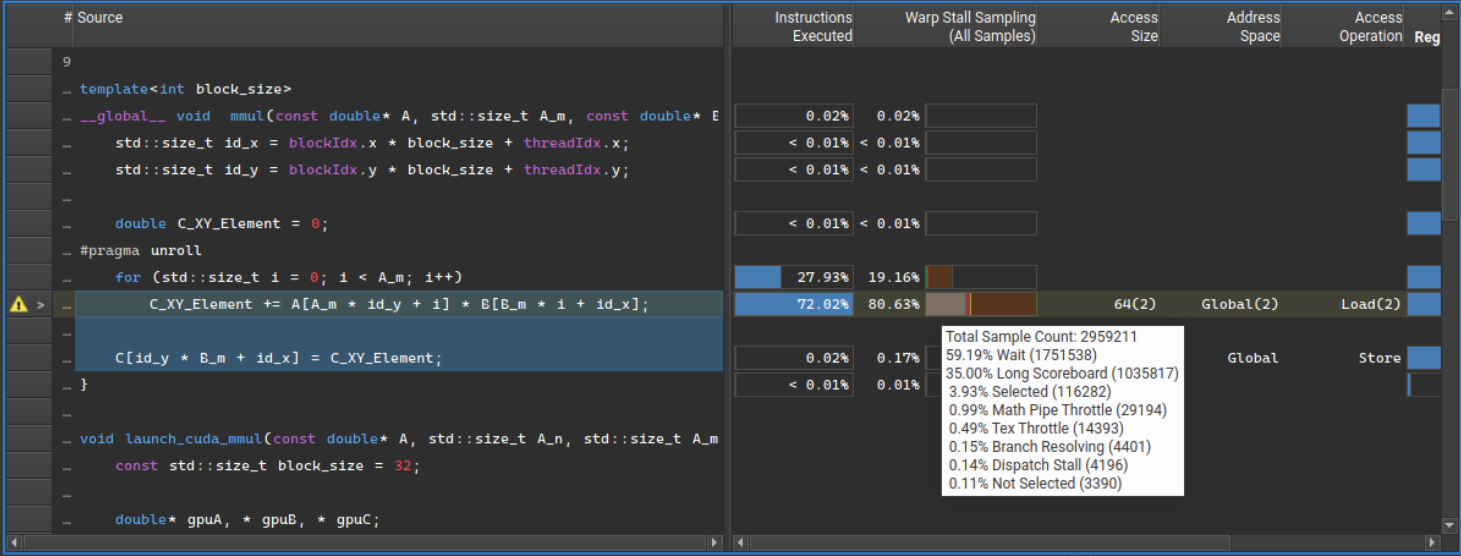
\includegraphics[width=1.0\textwidth]{img/native_warpstall.png}
  \caption{Нативный matmul source code.}
  \label{fig:image_label}
\end{figure}

На картинке видно, что достаточно трудоемкая строчка исходного кода показывает большую метрику warp stall.
Warp stall возникает, когда потоки в warp`e не могут выполнить инструкции 
из-за зависимостей данных, медленного доступа к памяти или ветвлений. 
Для того чтобы детальнее разобраться в вопросе необходимо взглянуть на 
ассемблерный код.

\newpage

\begin{figure}[h]
  \centering
  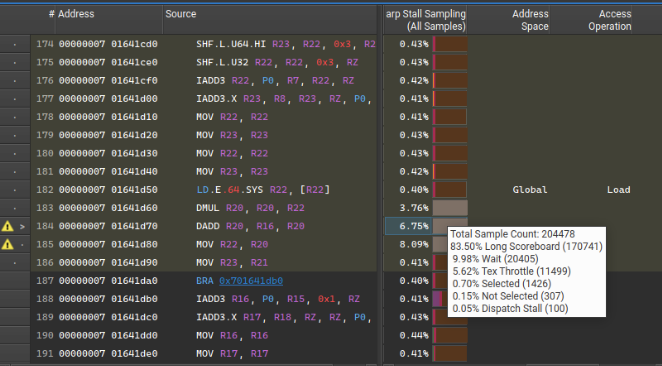
\includegraphics[width=1.0\textwidth]{img/native_asm.png}
  \caption{Нативный matmul asm. Warp stall (GM access)}
  \label{fig:image_label}
\end{figure}


В нашем случае видно что больше всего времени программа простаивает в ожидании инструкции LD (Доступ в глобальную памятью).
Для того чтобы уменьшить количество warp stall в данной ситуации, необходимо оптимизировать доступ к памяти, 
использовать shared memory и минимизировать зависимости между потоками.

Использование shared memory позволяет уменьшить количество обращений к 
глобальной памяти, предоставляя потокам более быстрый доступ к данным, 
которые используются совместно в пределах блока. 
Это особенно важно для операций, таких как матричное умножение, 
где элементы матриц часто многократно используются и могут быть 
эффективно предзагружены для повышения параллелизма 
и уменьшения затрат на доступ к памяти.

\newpage

\section{Оптимизация}
В данной секции мы сосредоточимся на оптимизации CUDA-кернела 
для матричного умножения (matmul), используя shared memory. 
Основная цель оптимизации заключается в значительном улучшении 
производительности за счет уменьшения задержек доступа к глобальной памяти, 
которая является относительно медленной по сравнению с памятью, 

Оптимизированная версия:

\vspace{10pt}
\begin{lstlisting}[language=CUDA, caption={optimized matmul}, label={code:cuda_matmul}]
  template<int block_size>
  __global__ void mmul(const double* A, std::size_t A_m, const double* B, std::size_t B_m, double* C) {
      int bx = blockIdx.x;
      int by = blockIdx.y;
      int tx = threadIdx.x;
      int ty = threadIdx.y;
      unsigned int wA = A_m;
      unsigned int wB = B_m;
      int aBegin = A_m * block_size * by;
      int aEnd = aBegin + wA - 1;
      int aStep = block_size;
      int bBegin = block_size * bx;
      int bStep = block_size * wB;
      float Csub = 0;
      for (int a = aBegin, b = bBegin; a <= aEnd; a += aStep, b += bStep) {
          __shared__ float As[block_size][block_size];
          __shared__ float Bs[block_size][block_size];
  
          As[ty][tx] = A[a + wA * ty + tx];
          Bs[ty][tx] = B[b + wB * ty + tx];
          __syncthreads();
  #pragma unroll
          for (int k = 0; k < block_size; ++k) {
              Csub += As[ty][k] * Bs[k][tx];
          }
          __syncthreads();
      }
      int c = wB * block_size * by + block_size * bx;
      C[c + wB * ty + tx] = Csub;
  }
\end{lstlisting}
\vspace{10pt} 
В этом коде потоки загружают блоки данных из матриц \(A\) и \(B\) в
shared memory, чтобы ускорить доступ и снизить задержки при
обращении к глобальной памяти. Затем выполняются параллельные вычисления
для каждого элемента результирующей матрицы \(C\), используя данные из
shared memory. Далее посмотрим на производительность данного решения.

\section{Тестирование оптимизированной версии}
Для начала посмотрим на source-assembly отчет и попробуем найти слабые места.

\begin{figure}[h]
  \centering
  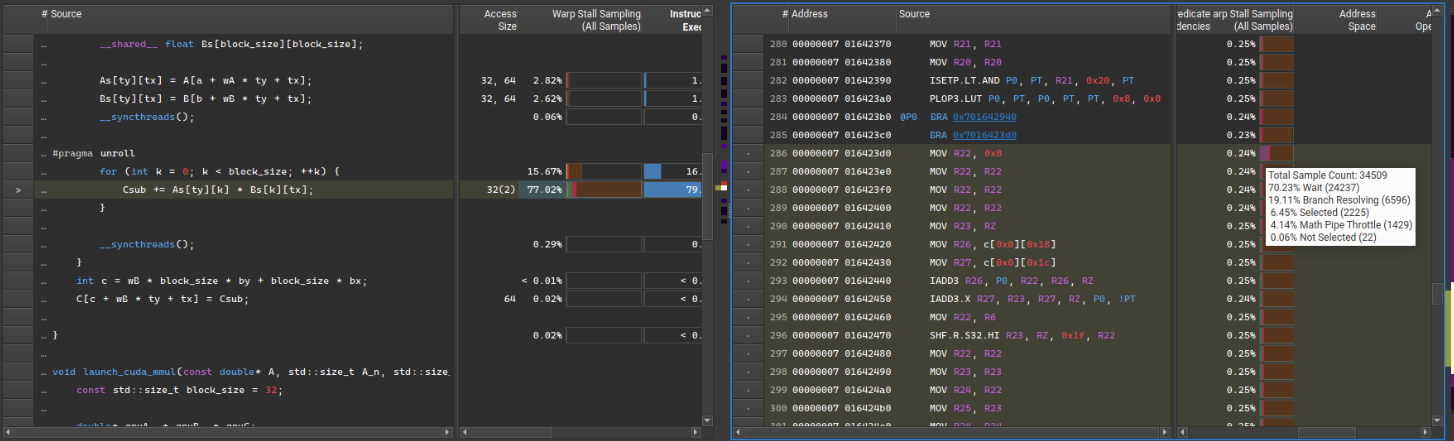
\includegraphics[width=1.0\textwidth]{img/optimized_sa.png}
  \caption{Оптимизированный matmul source-assembly. Wait barrier}
  \label{fig:image_label}
\end{figure}

В нашем случае видно что выделенная инструкция обладает достаточно большим Warp stall. 
Однако в нашей реализации необходимо наличие барьеров до и после доступов к shared memory
поэтому в данном случае очевидных оптимизаций нет.

\newpage

Теперь сравним производительность нативной версии и оптимизированной по нескольким показателям:

\begin{enumerate}
  \item Execution time: Время исполнения device части программы.
  \item SM Throughput: производительность одного Streaming Multiprocessor (SM).
  \item DRAM Throughput: скорость передачи данных между DRAM (Dynamic Random Access Memory) и вычислительными блоками GPU.
\end{enumerate}

\begin{table}[h]
  \centering
  \begin{tabular}{|c|c|c|}
  \hline
  Metric & Native & Optimized \\ \hline
  Execution time & 573.36us & 375.51us \\ \hline
  SM Throughput & 60\% & 88\% \\ \hline
  DRAM Throughput & 1,34\% & 1,93\% \\ \hline
  \end{tabular}
  \caption{Сравнение по характеристикам}
\end{table}

\newpage
Более подробное сравнение можно увидеть на картинках ниже.

\begin{figure}[h]
  \centering
  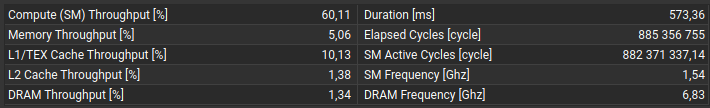
\includegraphics[width=1.0\textwidth]{img/native_summary.png}
  \caption{Summary. Нативный matmul}
  \label{fig:image_label}
\end{figure}

\begin{figure}[h]
  \centering
  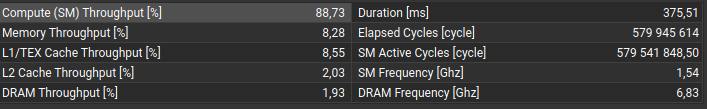
\includegraphics[width=1.0\textwidth]{img/optimized_summary.png}
  \caption{Summary. Оптимизированный matmul}
  \label{fig:image_label}
\end{figure}

\newpage
\section{Заключение}

Таким образом мы проанализировали основные проблемы, связанные с производительностью, 
такие как задержки доступа к глобальной памяти и низкий SM Throughput
и прелложили методы их устранения. Использование shared memory позволило 
значительно снизить количество обращений к медленной глобальной памяти и повысить общую эффективность вычислений
на 28\%. Также была увеличена эффективность доступа в глобальную память на 44\%.

Результаты экспериментов показали значительное улучшение времени выполнения операции матричного 
умножения на 52\%, что подтверждает эффективность примененной оптимизации. 

\section{Приложение}

Весь код, а так же отчеты о производительности в формате .ncu-rep можно найти в следующем репозитории: https://github.com/Poolce/cuda-perf-optimization

\end{document}